\chapter{Projekt systemu i opis narzędzi}
\label{DesignSystemChapter}
W poniższym rozdziale zostaną zaprezentowane kluczowe decyzje projektowe oraz założenia, jakie zostały przyjęte w toku prac nad implementacją systemu. Oprócz tego zostanie również przedstawiony opis narzędzi, które zostały wykorzystane do stworzenia aplikacji.

\section{Projekt systemu}
W fazie projektowania należy zdefiniować główne założenia projektowe oraz odpowiednio zaprojektować architekturę systemu. W dalszej części tego rozdziału zostaną omówione trzy kluczowe zagadnienia, jakie powstały w wyniku prac przeprowadzonych w ramach realizacji tej fazy.

\subsection{Problem do rozwiązania}
Zaprojektowany system powinien być zdolny do rozwiązania problemu uczenia konwolucyjnej sieci neuronowej, przeznaczonej do kierowania samochodem poruszającym się po wirtualnym torze wyścigowym. Sieć generuje komendy dla samochodu na podstawie obrazu z kamery umieszczonej wewnątrz pojazdu.

Trening sieci neuronowej ma się odbywać poprzez wykorzystanie metody uczenia maszynowego o nazwie \textbf{uczenie ze wzmocnieniem} (z ang. \textit{reinforcement learning}) \cite{deepRL:guide}. Jako algorytm uczący wykorzystano algorytm PPO \cite{ppo:opis}.

\subsection{Cele i założenia}
\begin{enumerate*}
\item Stworzony system powinien być możliwie prosty w obsłudze.
\item Po skończonym treningu, model sieci neuronowej ma być przechowywany w pliku o formacie ONNX \cite{onnx:website}. Plik z modelem musi być rozpoznawany w systemie, tak aby była możliwość ewaluacji wyuczonego modelu.
\item Konfiguracja treningu ma być tworzona w pliku tekstowym o zdefiniowanym formacie. Przy starcie treningu należy podać ścieżkę do pliku z konfiguracją.
\item System musi udostępniać możliwość podglądu ,,na żywo'' przebiegu trwającego treningu sieci neuronowej.
\end{enumerate*}

\subsection{Architektura systemu}
\label{SoftwareArchSection}
System jest złożony z dwóch głównych modułów, niezależnych od siebie: Środowiska Uczenia oraz narzędzia \texttt{mlagents\_learn}. Komunikacja między modułami odbywa się poprzez mechanizm zdefiniowany w zestawie Unity ML-Agents. Uproszczona wizualizacja systemu została zobrazowana na rysunku \ref{SystemArchitecture}. Aby dowiedzieć się więcej na temat każdego z modułów, należy zapoznać się z rozdziałem \ref{ImplementationChapter}-tym, gdzie znajduje się opis ich implementacji. \\

\begin{figure}[h]
\begin{center}
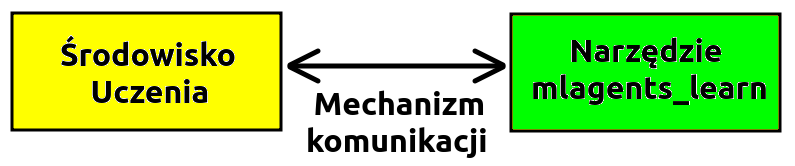
\includegraphics[width=15cm]{resources/figures/system_architecture.png}
\caption{Moduły systemu}
\label{SystemArchitecture}
\end{center}
\end{figure}

\section{Opis narzędzi}
Aby zaimplementować system, autor pracy musiał korzystać z pewnych narzędzi. \\
Poniżej znajduje się ich opis.

\subsection{Unity}
Jeden z najpopularniejszych silników gier \cite{unity:opis}, wspierający zdecydowaną większość platform dostępnych obecnie na rynku. Do tych platform należy zaliczyć: komputery klasy PC (Windows, MacOS, Linux), urządzenia mobilne (iOS, Android), konsole do gier (PlayStation 4, PlayStation 5, Xbox One, Nintendo Switch) oraz wiele innych. Pełna lista wspieranych platform jest dostępna na stronie dokumentacji silnika Unity \cite{unity:buildTargets}.

Warto również wspomnieć o bardzo atrakcyjnych warunkach licencyjnych - większość funkcji oferowanych przez silnik jest legalnie dostępna za darmo dla użytkowników, których roczny dochód nie przekracza 100 000 dolarów.

W Unity powstało wiele popularnych gier, takich jak:
\begin{enumerate*}
\item Pokémon Go,
\item Hearthstone: Heroes of Warcraft,
\item Firewatch,
\item The Forest,
\item Car Mechanic Simulator,
\item Gwint: Wiedźmińska Gra Karciana,
\item Syberia 3,
\item i wiele innych.
\end{enumerate*}

Ostatnią funkcją wartą uwagi jest moduł \textbf{Unity Asset Store}, który pozwala na publikowanie oraz pobieranie zarówno darmowych, jak i płatnych komponentów do wykorzystania w projektach silnika Unity. Komponenty mogą zawierać zasoby różnego typu, takie jak modele 3D, skrypty języka C\# lub pliki audio.

\subsection{C\#}
Język programowania stworzony przez firmę Microsoft jako konkurencja dla Javy \cite{csharp:opis}. Jest wysokopoziomowym, obiektowym językiem programowania, ściśle zintegrowanym z platformą .NET (pełniącą rolę frameworka oraz środowiska uruchomieniowego). Charakteryzuje się silnym, statycznym typowaniem. C\# pozwala na tworzenie aplikacji desktopowych (Windows, Linux, MacOS), webowych (poprzez użycie frameworka ASP.NET) oraz multiplatformowych aplikacji mobilnych (poprzez wykorzystanie narzędzia Xamarin). Obecnie jest to jeden z najpopularniejszych języków programowania.

\subsection{Unity ML-Agents}
\label{UnityMlSection}
Otwartoźródłowy zestaw narzędzi przeznaczony dla silnika Unity 3D \cite{unitymla:overview}. Został stworzony w celu ułatwienia treningu sieci neuronowych w środowiskach symulowanych komputerowo. Sieci neuronowe mogą być trenowane przy użyciu jednej z kilku możliwych metod uczenia maszynowego:
\begin{enumerate*}
\item Uczenie ze wzmocnieniem (z ang. \textit{reinforcement learning}) \cite{deepRL:guide}:
\begin{itemize*}
\item wykorzystując algorytm PPO \cite{ppo:opis};
\item wykorzystując algorytm SAC \cite{sac:opis};
\end{itemize*}
\item Uczenie przez imitację (z ang. \textit{imitation learning}) \cite{imitationLearning:article},
\item Neuroewolucja \cite{neuroevolution:primer},
\item Inna metoda uczenia maszynowego - zdefiniowana przez użytkownika.
\end{enumerate*}

Zestaw Unity ML-Agents jest złożony z pięciu podstawowych modułów:
\begin{enumerate*}
\item Środowisko Uczenia (z ang. \textit{Learning Environment}) - obejmuje scenę Unity oraz wszystkie obiekty znajdujące się na niej. Scena Unity dostarcza środowisko do generowania obserwacji, wykonywania działań i uczenia się.
\item Niskopoziomowe API języka Python (z ang. \textit{Python Low-Level API}) \cite{unitymla:pythonapi} - cytując dokumentację zestawu Unity ML-Agents \cite{unitymla:overview}, jest to ,,\textit{niskopoziomowy interfejs programistyczny, służący do komunikacji ze Środowiskiem Uczenia. API Pythona istnieje jako osobny byt (niezależny od silnika Unity), komunikujący się ze sceną Unity dzięki Zewnętrznemu Komunikatorowi. API jest zaimplementowane w języku Python i zawarte w pakiecie o nazwie} \texttt{mlagents\_envs}''.
\item Zewnętrzny Komunikator (z ang. \textit{External Communicator}) - odpowiedzialny za komunikację pomiędzy Środowiskiem Uczenia a Niskopoziomowym API języka Python.
\item Trenerzy Pythona (z ang. \textit{Python Trainers}) - zestaw algorytmów uczenia maszynowego, napisanych w języku Python. Algorytmy te są częścią pakietu \texttt{mlagents}, w skład którego wchodzi także konsolowe narzędzie o nazwie \texttt{mlagents-learn}, odpowiedzialne za obsługę wszystkich metod treningu wspieranych przez Unity ML-Agents.
\item Gym Wrapper - opisany w dokumentacji zestawu \cite{unitymla:gymWrapper}, zupełnie nieistotny dla dalszych rozważań.
\end{enumerate*}

Komponenty zestawu Unity ML-Agents zostały zilustrowane na rysunku \ref{UnityMlaComponents}, na którym narysowano wszystkie komponenty poza Gym Wrapperem.

Poprawnie skonfigurowane Środowisko Uczenia musi zawierać następujące elementy:
\begin{enumerate*}
\item Co najmniej jednego Agenta (z ang. \textit{Agent}). Agent to komponent dołączany do obiektu klasy \texttt{GameObject}, umiejscowionego na scenie Unity. Każdy Agent jest instancją klasy dziedziczącej po klasie \texttt{Agent} i jest odpowiedzialny za przygotowanie Obserwacji dla sieci neuronowej, wykonywanie Akcji generowanych przez sieć neuronową oraz obliczanie wartości sygnałów Nagrody.
\item Co najmniej jednego Zachowania (z ang. \textit{Behavior}). Zachowanie definiuje określone atrybuty Agenta, takie jak liczba i rodzaj wykonywanych Akcji. Każde Zachowanie jest jednoznacznie identyfikowane poprzez pole \texttt{Behavior Name}. \\
Istnieją trzy rodzaje Zachowań:
\begin{itemize*}
\item Zachowanie Uczące (z ang. \textit{Learning Behavior}) - Zachowanie, którego Agent musi się wyuczyć. Tego Zachowania używamy podczas treningu sieci neuronowych;
\item Zachowanie Heurystyczne (z ang. \textit{Heuristic Behavior}) - Zachowanie zdefiniowane przez reguły zapisane bezpośrednio w kodzie źródłowym. Przydatne m.in. przy testowaniu nowego Środowiska Uczenia przed rozpoczęciem treningu sieci.
\item Zachowanie Wnioskujące (z ang. \textit{Inference Behavior}) - Zachowanie wykorzystujące wytrenowany model sieci neuronowej. W gruncie rzeczy, Zachowanie Uczące po skończonym treningu sieci neuronowej zmienia się w Zachowanie Wnioskujące.
\end{itemize*}
\end{enumerate*}

\begin{figure}[h]
\begin{center}
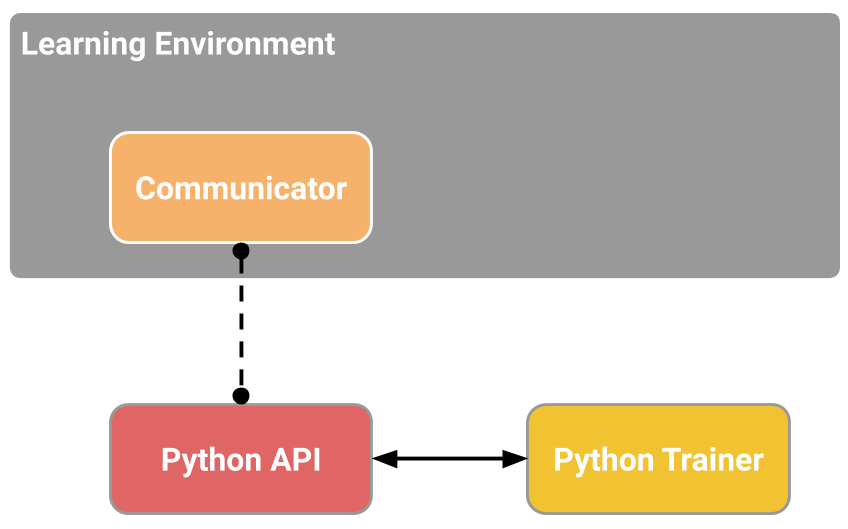
\includegraphics[width=15cm]{resources/figures/learning_environment_basic.png}
\caption{Diagram komponentów Unity ML-Agents}
\source{https://github.com/Unity-Technologies/ml-agents/blob/release_19_docs/docs/ML-Agents-Overview.md}
\label{UnityMlaComponents}
\end{center}
\end{figure}

Każdy Agent musi być powiązany z dokładnie jednym Zachowaniem, a Zachowanie może być połączone z więcej niż jednym Agentem. Agenci działający wedle tej samej logiki powinni być powiązani z tym samym Zachowaniem. To wcale nie oznacza, że wszyscy Agenci powiązani z tym samym Zachowaniem muszą współdzielić ze sobą te same Obserwacje, Akcje i Nagrody.

Rysunek \ref{UnityMlaExample} przedstawia przykładowy diagram zależności Agentów z Zachowaniami w Środowisku Uczenia. Agenci \texttt{A1} i \texttt{A2} są podłączeni do Zachowania Uczącego. Agenci \texttt{C1} i \texttt{D1} są podłączeni odpowiednio do Zachowania Wnioskującego i Heurystycznego.

Opisując narzędzie Unity ML-Agents, należałoby również wspomnieć kilka słów o samym Agencie. Każdy Agent wykonuje cyklicznie trzy czynności: generuje Obserwacje, wykonuje zlecone Akcje i oblicza wartość Nagrody. Omówmy każdy z tych elementów:

\newpage
\begin{figure}[h]
\begin{center}
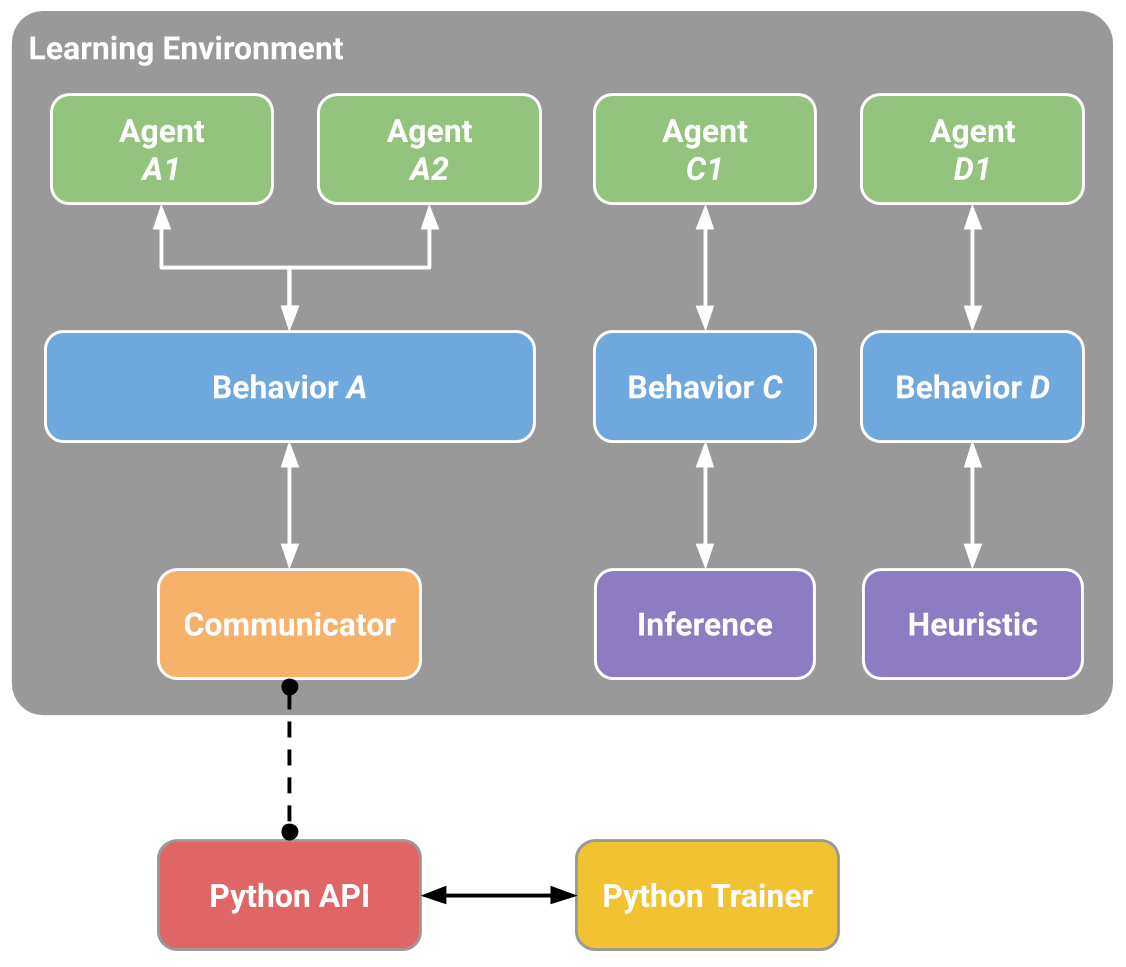
\includegraphics[width=15cm]{resources/figures/learning_environment_example.png}
\caption{Przykład relacji Agentów z Zachowaniami w Środowisku Uczenia}
\source{https://github.com/Unity-Technologies/ml-agents/blob/release_19_docs/docs/ML-Agents-Overview.md}
\label{UnityMlaExample}
\end{center}
\vspace{-1cm}
\end{figure}

\begin{enumerate*}
\item Obserwacje (z ang. \textit{Observations}) - zestaw danych wejściowych, niezbędnych do wykonania zleconego Agentowi zadania. Obserwacje mogą być generowane na kilka sposobów:
\begin{itemize*}
\item Nadpisanie metody \texttt{Agent.CollectObservations()} i przesłanie obserwacji do dostarczonego (przez parametr metody) obiektu klasy \texttt{VectorSensor}. Ten sposób najlepiej wykorzystać do aspektów środowiska, które można opisać numerycznie i niewizualnie.
\item Dodanie atrybutu \texttt{[Observable]} do pól i właściwości Agenta. Atrybut \\ \texttt{[Observable]} wspiera obecnie podstawowe typy danych (takie jak  \texttt{int}, \texttt{float} czy \texttt{bool}), jak również klasy \texttt{Vector2}, \texttt{Vector3}, \texttt{Vector4}, \texttt{Quaternion} oraz typy enumeracyjne.
\item Implementacja interfejsu \texttt{ISensor}, korzystając z \texttt{SensorComponent} dołączanego do Agenta. Obecnie istnieje kilka implementacji komponentu \texttt{SensorComponent} dostarczanych przez API zestawu Unity ML-Agents. Najważniejsze z nich to:
\begin{itemize*}
\item \texttt{CameraSensorComponent} - używa obrazów z kamery jako obserwacji;
\item \texttt{RenderTextureSensorComponent} - używa zawartości \texttt{RenderTexture} \cite{unity:renderTexture} jako obserwacji;
\item \texttt{RayPerceptionSensorComponent} - używa informacji z zestawu promieni (z ang. \textit{ray casts}) jako obserwacji.
\end{itemize*}
\end{itemize*}
\item Akcje (z ang. \textit{Actions}) - instrukcje zachowań, które Agent powinien wykonać. Istnieją dwa typy Akcji - Ciągłe (z ang. \textit{Continuous}) oraz Nieciągłe (z ang. \textit{Discrete}). Wszystkie Akcje muszą być zdefiniowane w metodzie \texttt{OnActionReceived()}. Akcje Ciągłe to wartości ze zbioru liczb rzeczywistych, podczas gdy Akcje Nieciągłe są wartościami całkowitymi.
\item Nagrody (z ang. \textit{Rewards}) - informacja zwrotna, pozwalająca ocenić jak dobre (lub złe) są Akcje wykonywane obecnie przez Agenta. System Nagród jest najważniejszym elementem w uczeniu ze wzmocnieniem, ponieważ sposób jego skonstruowania ma decydujący wpływ na to, czy trening sieci neuronowej się powiedzie.
\end{enumerate*}

\subsection{Vehicle Physics Pro}
\label{VppSection}
Zaawansowany zestaw do symulacji pojazdów dla silnika Unity 3D. VPP zapewnia wydajny, w pełni realistyczny i dokładny model dynamiki dla niemal każdego typu pojazdu i konfiguracji. Większość aspektów symulacji podlega możliwościom dostosowania do potrzeb użytkownika. W skład zestawu wchodzą m.in. \cite{vpp:features}:
\begin{enumerate*}
\item Wierne odwzorowanie pracy podzespołów pojazdu, obejmujące m.in.:
\begin{itemize*}
\item pracę silnika (spalinowego lub elektrycznego),
\item pracę skrzyni biegów (manualnej lub automatycznej),
\item pracę układu kierowniczego;
\end{itemize*}
\item Symulacja systemów wspomagania jazdy, w tym:
\begin{itemize*}
\item ABS (Anti-lock Braking System),
\item TCS (Traction Control System),
\item ESC (Electronic Stability Control);
\end{itemize*}
\item Liczne rozszerzenia i dodatki, takie jak:
\begin{itemize*}
\item efekty wizualne (np. animacja deski rozdzielczej),
\item efekty dźwiękowe (np. dźwięk silnika),
\item zaawansowana diagnostyka pojazdu, obejmująca m.in. pomiary telemetryczne,
\item system nagrywania, odtwarzania i zapisu powtórek wideo;
\end{itemize*}
\item System zniszczeń wizualnych i mechanicznych;
\item Obsługa szerokiej gamy urządzeń wejściowych, takich jak gamepady czy kierownice do gier wyścigowych;
\item Szczegółowa dokumentacja.
\end{enumerate*}

\subsection{Netron}
\label{NetronOpis}
Przeglądarka sieci neuronowych \cite{netron:github}. Netron posiada wsparcie dla wielu popularnych technologii wykorzystywanych w uczeniu maszynowym, takich jak ONNX, Keras, czy Barracuda. Ten program został wykorzystany do wizualizacji modelu wytrenowanej sieci neuronowej, otrzymanej w wyniku przeprowadzenia serii eksperymentów obliczeniowych.

\subsection{Wykorzystane wersje narzędzi}
\begin{enumerate*}
\item Unity - 2020.3.28f
\item C\# - Mono 6.12.0.122
\item Unity ML-Agents - 0.28.0
\item Vehicle Physics Pro - 9.2
\item Netron - 5.7.6
\end{enumerate*}

\subsection{Specyfikacja techniczna komputera}
\label{ComputerTechSpecs}
Oto specyfikacja techniczna komputera, na którym autor wykonał całą pracę związaną z implementacją systemu oraz przeprowadzeniem eksperymentów obliczeniowych:
\begin{enumerate*}
\item Marka i model komputera - Dell Inspiron 7559 \cite{dellInspiron:specs}
\item Procesor - Intel® Core™ i7-6700HQ (2.6 GHz) \cite{intelCpu:specs}
\item Pamięć RAM - SODIMM DDR3 Synchronous 1600 MHz (32 GB)
\item Karty graficzne:
\begin{itemize*}
\item nVidia GeForce GTX 960M \cite{nvidiaGPU:specs}
\item Intel HD Graphics 530
\end{itemize*}
\item Dysk - PLEXTOR PX-512M7 (SSD 512 GB)
\item System operacyjny - Linux Mint 19.1 Tessa
\end{enumerate*}